% \documentclass[aspectratio=169,notes]{beamer}
\documentclass[aspectratio=169]{beamer}
\usetheme[faculty=phil]{fibeamer}
\usepackage{polyglossia}
\setmainlanguage{english} %% main locale instead of `english`, you
%% can typeset the presentation in either Czech or Slovak,
%% respectively.
\setotherlanguages{russian} %% The additional keys allow
%%
%%   \begin{otherlanguage}{czech}   ... \end{otherlanguage}
%%   \begin{otherlanguage}{slovak}  ... \end{otherlanguage}
%%
%% These macros specify information about the presentation
\title[Theoretical Mechanics]{Week HW 5, PART [Non]INERT} %% that will be typeset on the
\subtitle{Particle dynamics for inertial systems\\
Particle dynamics for noninertial systems\\
\ 
         } %% title page.
\author{Oleg Bulichev}
%% These additional packages are used within the document:
\usepackage{ragged2e}  % `\justifying` text
\usepackage{booktabs}  % Tables
\usepackage{tabularx}
\usepackage{tikz}      % Diagrams
\usetikzlibrary{calc, shapes, backgrounds}
\usepackage{amsmath, amssymb}
\usepackage{url}       % `\url`s
\usepackage{listings}  % Code listings
% \usepackage{subfigure}
\usepackage{floatrow}
\usepackage{subcaption}
\usepackage{mathtools}
\usepackage{todonotes}
\usepackage{fontspec}
\usepackage{multicol}
\usepackage{pdfpages}
\usepackage{wrapfig}
\usepackage{animate}
\usepackage{booktabs}
\usepackage{multirow}
% \usepackage{graphicx}
\usepackage{colortbl}

\graphicspath{{resources/}}
\frenchspacing

\setbeamertemplate{caption}[numbered]
\usetikzlibrary{graphs}

% \usepackage[backend=biber,style=ieee,autocite=footnote]{biblatex}
% \addbibresource{biblio.bib}
% \DefineBibliographyStrings{english}{%
%   bibliography = {References},}

\newcommand{\oleg}[2][] {\todo[color=red, #1] {OLEG:\\ #2}}
\newcommand{\fbckg}[1]{\usebackgroundtemplate{\includegraphics[width=\paperwidth]{#1}}}%frame background

\usepackage[framemethod=TikZ]{mdframed}
\newcommand{\dbox}[1]{
\begin{mdframed}[roundcorner=3pt, backgroundcolor=yellow, linewidth=0]
\vspace{1mm}
{#1}
\vspace{1mm}
\end{mdframed}
}

\begin{document}
\setlength{\abovedisplayskip}{0pt}
\setlength{\belowdisplayskip}{0pt}
\setlength{\abovedisplayshortskip}{0pt}
\setlength{\belowdisplayshortskip}{0pt}

\fbckg{fibeamer/figs/title_page.png}
\frame[c]{\setcounter{framenumber}{0}
    \usebeamerfont{title}%
    \usebeamercolor[fg]{title}%
    \begin{minipage}[b][6.5\baselineskip][b]{\textwidth}%
        \textcolor{black}{\raggedright\inserttitle}
    \end{minipage}
    % \vskip-1.5\baselineskip

    \usebeamerfont{subtitle}%
    \usebeamercolor[fg]{framesubtitle}%
    \begin{minipage}[b][3\baselineskip][b]{\textwidth}
        \raggedright%
        \insertsubtitle%
    \end{minipage}
    \vskip.25\baselineskip
}
%   \frame[c]{\maketitle}

\fbckg{fibeamer/figs/common.png}


\begin{frame}[t]{Task 1 (Coding)}
  \vspace*{-0.4cm}
  \scriptsize
\textbf{  The legend shall speak} that this situation was in WW2. There are two actors in this story: a sniper and an officer. Both knew about each other's existence. There was a river between them. The officer was always sitting in a trench, but the sniper knew his location and already calculated the distance to the target ($L\ meters$).

  After a while cargo ship appeared, which blocked the direct vision of the trench. The officer decided to stand up to stretch his legs. The sniper assumed that it might happened and make a shot, hitting the officer. Let's check this story.

\textbf{Formal description:} Considering the bullet as a material point and taking into account its weight and the force of wind resistance, we need to solve the following problems:
  \begin{itemize}
    \item Find the $\alpha$ (initial angle of overhang) that is required to hit the target. Output the value in degrees.
    \item At this angle, what is the maximum height the bullet will reach? Output the value.
    \item Plot $y(x)$, $F_c(t)$.
  \end{itemize}

  \vspace*{-0.3cm}
    \begin{minipage}{0.7\textwidth}    
      The problem should be solved in 2 ways. When air resistance is not taken into account, and when $F_c(v^2)=-kv \vec{v}$. The second problem can only be solved by numerical integration.
      
      All specifications about Mosin rifle such as bullet weight $m$, bullet velocity at departure $v_0$, effective firing distance are taken from the official documentation.
      
      $m=13.6\ g, L=1500\ m, k=1.3 \cdot 10^{-5}, v_0=870\ m/s$.
    \end{minipage}
    \begin{minipage}{0.29\textwidth}
      \vspace*{-0.6cm}
      \begin{figure}[H]
        \centering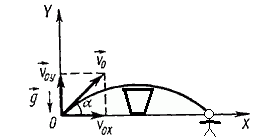
\includegraphics[height=6cm,width=1\textwidth,keepaspectratio]{HW5_1}
        \caption*{Task 1}
      \end{figure}
    \end{minipage}
  \end{frame}
  
  \begin{frame}[t]{Task 2 (Coding)}
    \vspace*{-0.5cm}
    \begin{minipage}{0.6\textwidth}
      \scriptsize
      A particle $M$ (mass $m$) is moving inside of the cylindrical channel of the moving object $D$. The object $D$ has a radius $r$. No friction between $M$ and $D$.
  
      Determine the equation of the relative motion of this particle $x=f(t)$. Also you need to find the pressure force the particle acting on the channel wall.
      
      At the end, you should provide:
      \begin{enumerate}
          \item simulate this mechanism (obtain all positions);
          \item show all acceleration components, inertial forces, gravity force and $N$;
          \item plot of the particle $x(t)$, till the time, while point won't leave the channel;
          \item plot $N(t)$ , till the time, while point won't leave the channel.
      \end{enumerate}
      
      Needed variables:\\
      $m=0.02,\ \omega=\pi,\ a = 60,\ \alpha=45^\circ$;\\
      Initial conditions: $t_0=0,\ x_0=0,\ \dot{x}_0=0.4$.
    \end{minipage}
    \begin{minipage}{0.39\textwidth}
      \vspace*{-0.3cm}
      \begin{figure}[H]
        \centering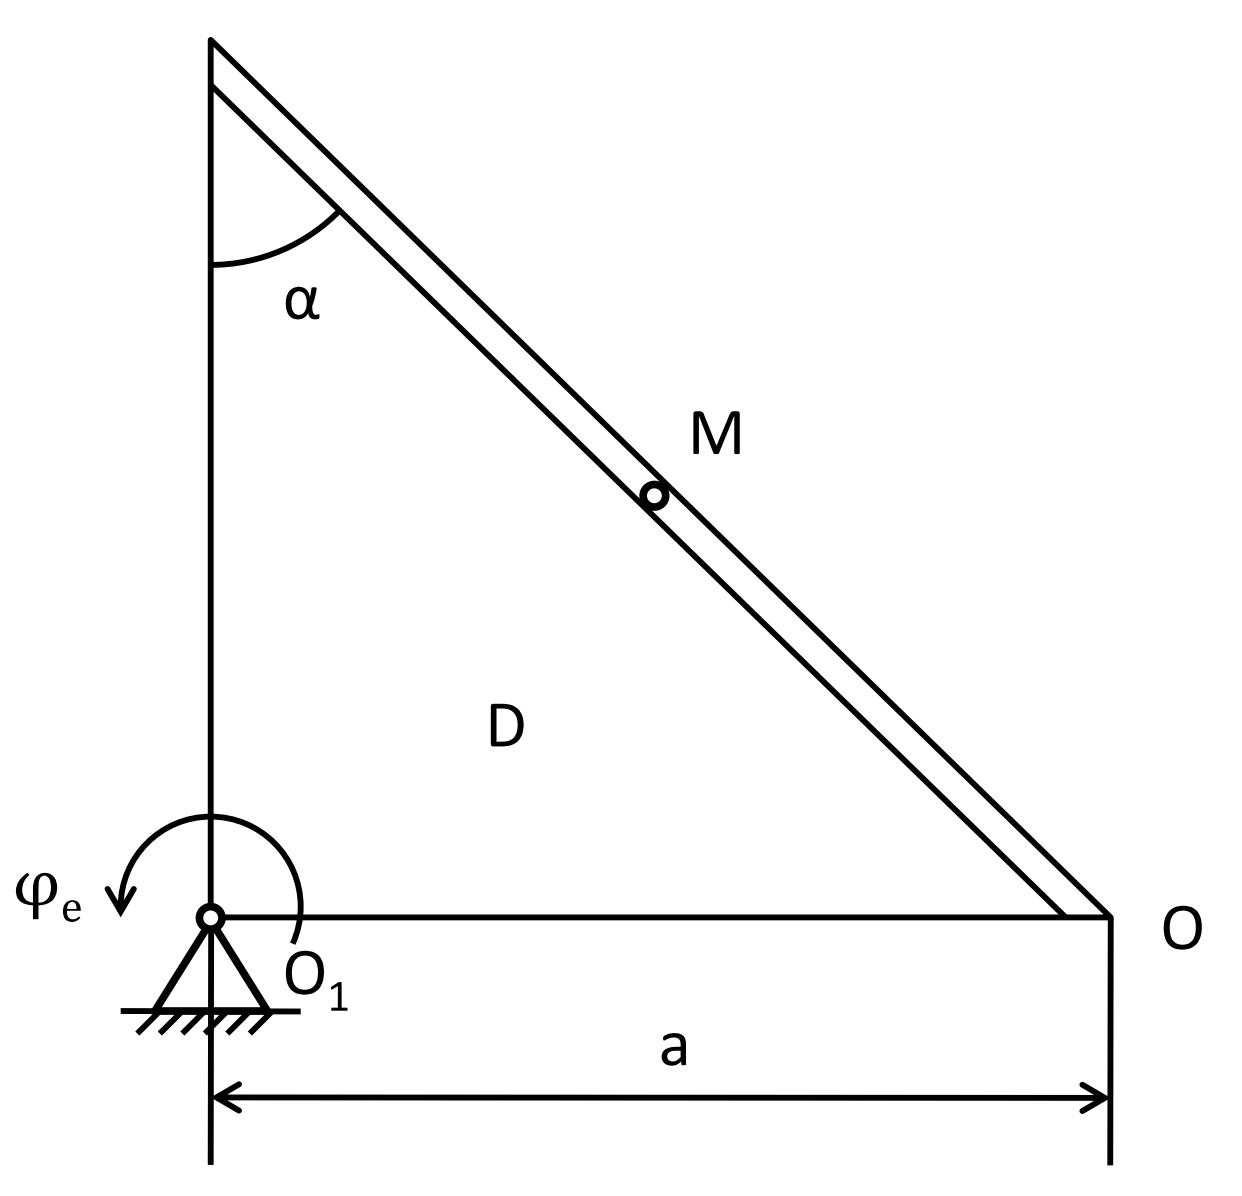
\includegraphics[height=6cm,width=1\textwidth,keepaspectratio]{HW3_2}
        \caption*{ Task 2\\ (Yablonskii (eng) D4)}
      \end{figure}
    \end{minipage}
  \end{frame}

\fbckg{fibeamer/figs/last_page.png}
\frame[plain]{}
\end{document}